%!TEX root = ../rapport.tex

\chapter{Existing Visualizations of the Lambda Calculus}

In this chapter we will discuss what already exists in areas related to our
project. First of all we have examples where lambda calculus has been
visualized, both using a piece of software, but also how lambda terms in
theory can be visualized. We will secondly discuss general visualization using
directed and semi-directed graphs.

We have not in our research found anything exactly similar to our thesis.
There does exist many examples where a given reduction has been visualized,
but never in a way giving a complete insight into the evaluation of the lambda
term. We have been able to find 9 examples of previous work related to our
work, and in the following section we will focus on two of them:

\begin{itemize}
	\item A Visual Lambda Calculus \cite{Citrin+Hall+Zorn+1995a}.
	\item Reduction graphs in the lambda calculus \cite{VenturiniZilli1984251}.
	\item Orders, reduction graphs and spectra \cite{297368}.
	\item Standard ML on the Web server: Visualizing Lambda Calculus Reduction \cite{Sestoft96standardml}.
	\item TILC: The Interactive Lambda-Calculus Tracer \cite{DBLP:journals/entcs/RuizV09}.
	% FIXME Hvad er det der overhovedet?
	% \item Visual Lambda \cite{visual-lambda}. 
	\item Lambda Animator \cite{lambdaAnimatorThyer}.
	\item Alligator Eggs - A Puzzle Game \cite{Alligator}.
	\item Animated Lambda Calculus Evaluator \cite{AnimatedLambdaCalculusEvaluator}.
\end{itemize}

% You can quantify the differentiations, from our project to these examples, by mainly two things:

The work we present differentiates itself from the previous work by mainly two
things:

\begin{itemize}
	\item It is currently not possible to get a complete overview of all
	      the reductions and thereby get an understanding of how the lambda
	      term evaluate ``over time''.
	\item Secondly, non existing visualizations has been capable of doing
	      it beautifully.
\end{itemize}

\section{Alligator Eggs -- A Puzzle Game by Bret Victor}

The ``Alligator Eggs - A Puzzle Game'' \cite{Alligator} is a ``fun'' and
children-like way of visualizing $\beta$-reductions of a lambda term. It was
originally not intended to be a computer program; the author instead designed
a set of drawings meant to be printed and cut out. This way, the visualization
can be used as a game. It visualizes the syntactic structure of lambda
terms, and the allowed ``moves'' in the game correspond to $\alpha$-conversion or
$\beta$-reduction.

The game uses a simple graphical alphabet:
\begin{description}
	\item[A hungry alligator] represents a lambda abstraction. The symbol can
	have different colors, analogously to variable names in ordinary lambda calculus.
	\item[An old alligator] is a parenthesis. It can only be white.
	\item[An egg] is a variable. It, too, can take on different colors.
\end{description}
Alligators are organized vertically into ``families''. The different families
are organized horizontally next to each other, and they are guarded by either an
old or a hungry alligator. The old alligator only concerns itself with
guarding, while the hungry alligator also has one or more eggs associated. If
an alligator and an egg are associated with each other, they have the same
color. It is straightforward to see the analogy to lambda terms.

With this alphabet, the rules are defined as follows:
\begin{description}
	\item[The Eating Rule] states that the topmost hungry alligator of a family can
	eat the family in front of it. When it does this it dies, but the eaten family
	is resurrected in its entirety from all the eggs associated with the hungry, dead
	alligator. This rule corresponds to a $\beta$-reduction. 
	\item[The Color Rule] states, that if an eaten family contains alligators and eggs
	in the same color as some alligators or eggs in the eating family, these must change colors
	to some new, unused color. This rule corresponds to an $\alpha$-conversion.
	\item[The Old Age Rule] states, that if the topmost alligator of a family is
	an old alligator, this alligator may die and nothing will happen. This is in analogy
	to the convention, that outermost parentheses in lambda terms are removed.
\end{description}

In figure \ref{fig:images_alligatorEat} we can see the Eating Rule in use. The
green alligator will eat whatever is in front of it. In this case it will eat
the yellow alligator and its yellow egg. After the green alligator has eaten
the yellow alligator and egg, it will die and its egg will hatch into what it
has eaten. ``The miracle of life'', as the author calls it. This so-called
``miracle'' is in our profane terminology called a $\beta$-reduction, as
mentioned above.

\begin{figure}[htbp]
	\centering
		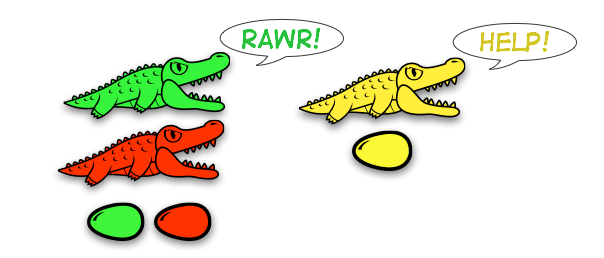
\includegraphics[width=2in]{../images/alligatorEat.png}
	\caption{A reduction visualized as an alligator eating}
	\label{fig:images_alligatorEat}
\end{figure}

In figure \ref{fig:images_alligatorOld} we can see an example of the old age
rule. In figure \ref{fig:images_alligatorOld} (a) the old alligator guards
more than one alligator and therefore works as a parenthesis. Now the green
alligator eats the red alligator. We can now in figure
\ref{fig:images_alligatorOld} (b) see that the old alligator only has the red
alligator to guard, which is the reason it now will die. In normal
mathematical words, this means that the parenthesis only concludes one element
and therefore is useless. Figure \ref{fig:images_alligatorOld} (c) shows the
end result with the old alligator dead.

\begin{figure}[htbp]
	\centering
		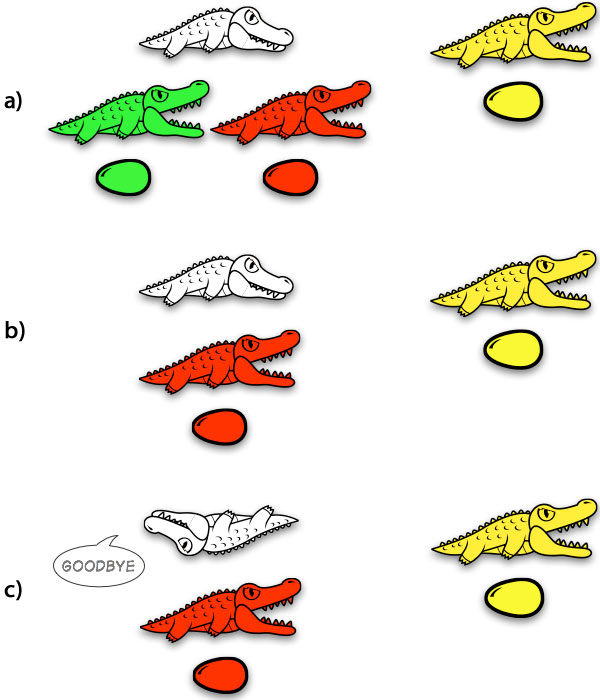
\includegraphics[width=2in]{../images/alligatorOld.jpg}
	\caption{Example of the old age rule}
	\label{fig:images_alligatorOld}
\end{figure}

``Alligator Eggs - A Puzzle Game'' does not deal with the same kind of
visualization tasks that we do in this project. It basically presents a
creative way of drawing syntax trees and a new, carnivorous terminology for
the transformations in the lambda calculus. 

The game has been implemented as a Java program, so that one does not need to
actually print out the alligators. (\cite{AlligatorTool})

\section{Lambda Animator by Mike Thyer}
The ``Lambda Animator'' is a representation of lambda terms in tree
form. It is implemented in Java and available online via a Java Applet (\cite{lambdaAnimatorThyer}).
\begin{figure}[!htbp]
	\centering
		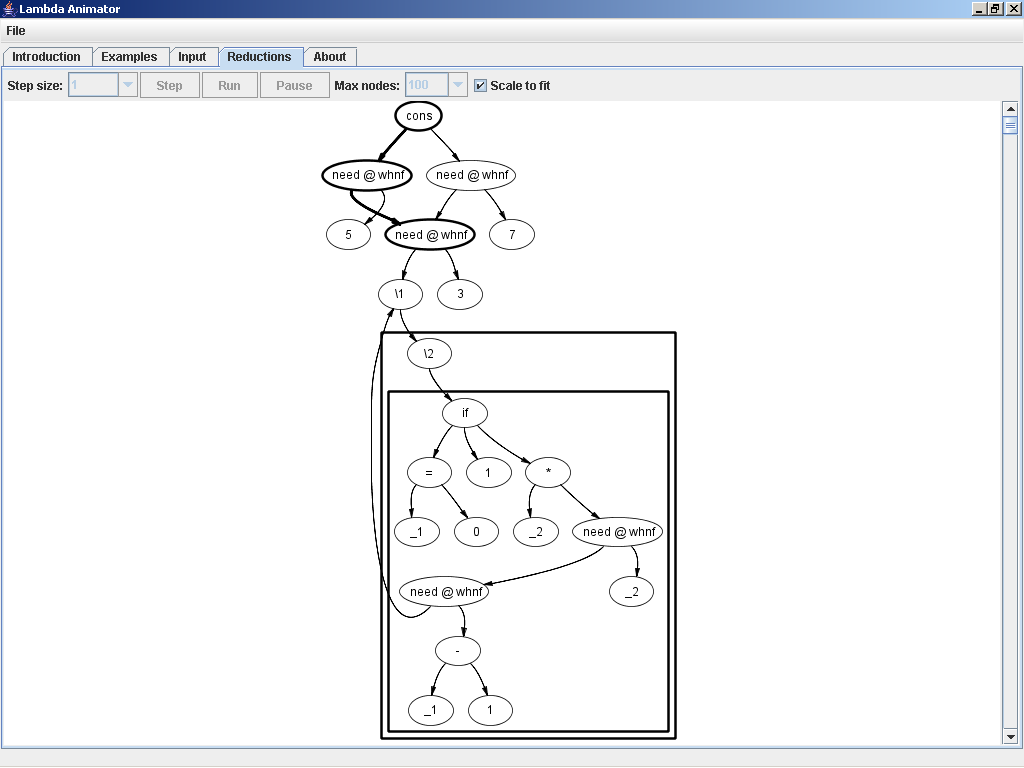
\includegraphics[scale=0.1]{../images/lambdaAnimator.png}
	\caption{Screenshot of the Lambda Animator tool}
	\label{fig:images_lambdaAnimator}
\end{figure}

The Animator does not seem very smooth and does not produce graphs that are
neither pretty nor especially visually informative. It uses extremely simple
graphics and does not fulfill our ``pretty'' criteria. The implementation in
the form of a Java applet does have some advantages in terms of easy access to
the tool.

It can give an reasonable overview when the lambda terms are not to complex.
In figure \ref{fig:images_lambdaAnimatorReduction} there is an example of a
simple $\beta$-reduction.

\begin{figure}[!htbp]
	\centering
		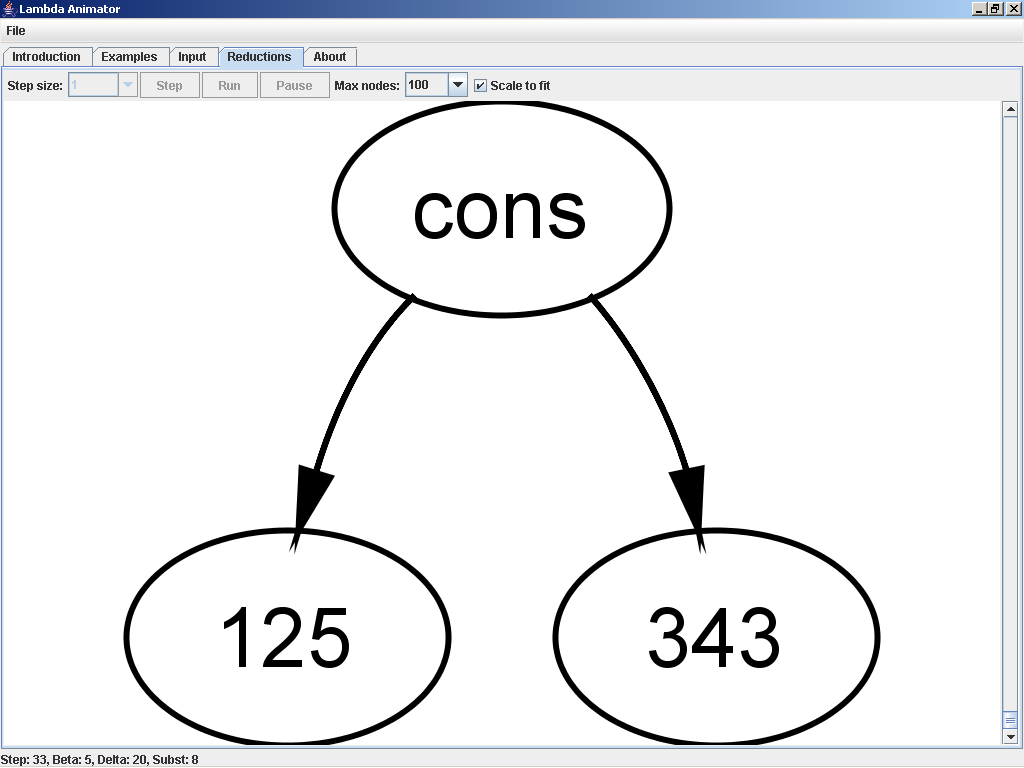
\includegraphics[scale=0.25]{../images/lambdaAnimatorReduction.png}
	\caption{Example of a simple $\beta$-reduction in the Lambda Animator}
	\label{fig:images_lambdaAnimatorReduction}
\end{figure}


\begin{figure}[!htbp]
	\centering
		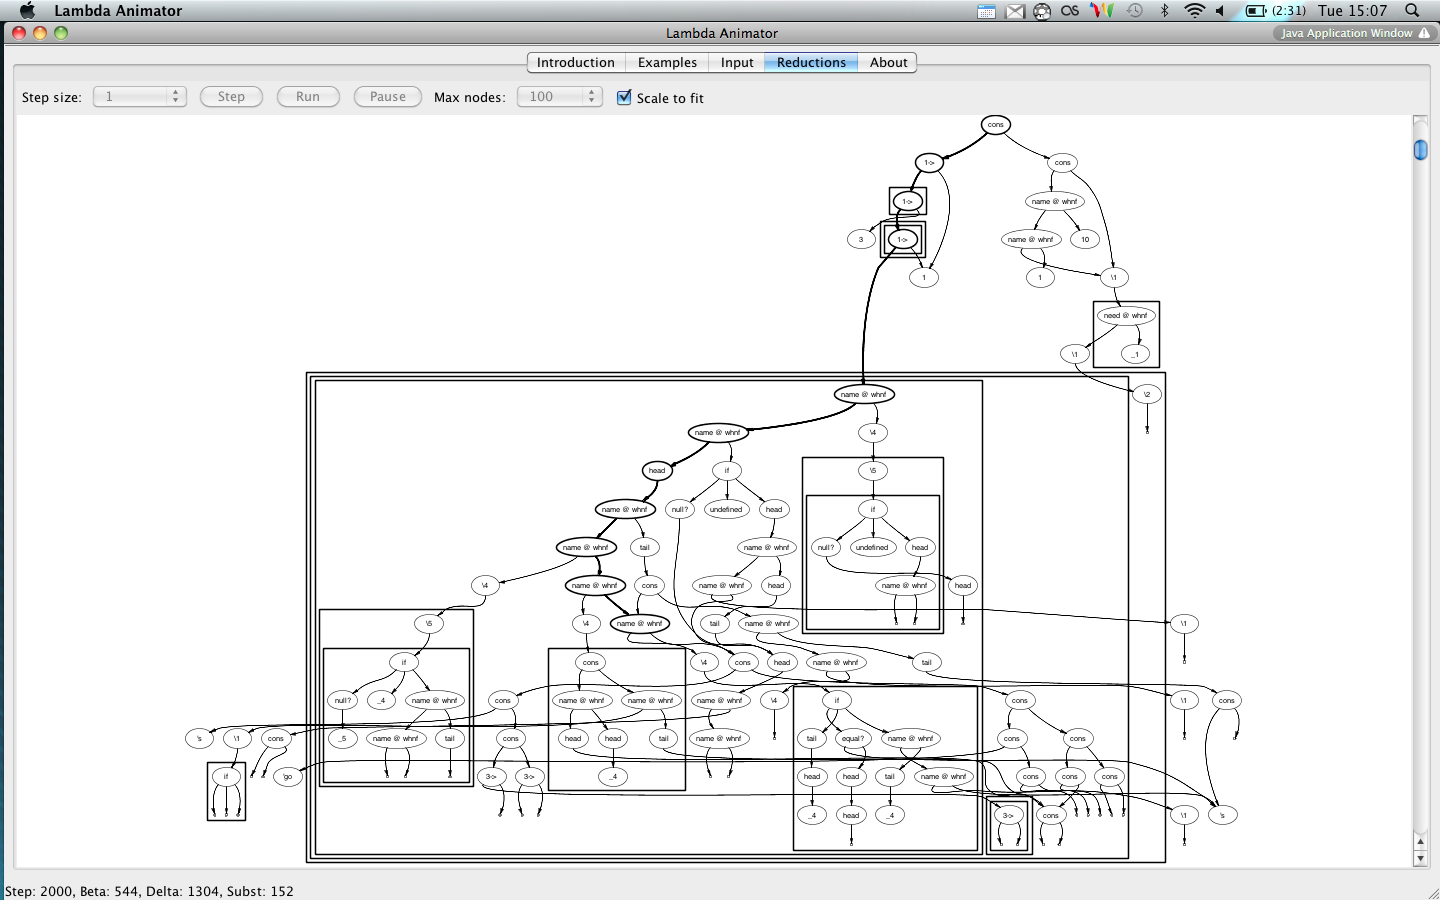
\includegraphics[scale=0.25]{../images/lambdaAnimatorComplex.png}
	\caption{Complex example in the Lambda Animator}
	\label{fig:images_lambdaAnimatorComplex}
\end{figure}

When you are dealing with more complex lambda terms it easily gets chaotic.
In figure \ref{fig:images_lambdaAnimatorComplex} there is another example, in
which one can see that the informativeness seems to drastically degrade when
the term complexity is increasing.

\section{Textual reduction}
Textual reduction ?

